\chapter{Petri Net Elements: Core Data Model}
\label{chap:petri-net-elements}

In the previous chapter, we explored the \texttt{UiService}, which manages \textit{what} the user is doing. This chapter focuses on \textit{what} the user is working with: the \textbf{Petri Net Elements}---the fundamental data objects that define the structure and behavior of any Petri net in our application.

\section{Problem Statement}
\label{sec:elements-problem}

To model a process like ``sending a letter,'' we need to represent:
\begin{itemize}
    \item \textbf{States}: The letter is unstamped, stamped, or mailed
    \item \textbf{Actions}: Stamp the letter, mail the letter
    \item \textbf{Flow}: How actions connect states
\end{itemize}

The \textbf{Petri Net Elements} are the fundamental building blocks that answer these questions. They are the ``nouns'' (states/conditions), ``verbs'' (actions/events), and ``arrows'' (connections) of our process models.

\section{Core Building Blocks}
\label{sec:elements-overview}

Petri nets consist of three element types:

\begin{table}[htb]
    \centering
    \begin{tabular}{llll}
        \toprule
        \textbf{Element} & \textbf{Visual} & \textbf{Represents} & \textbf{Analogy} \\
        \midrule
        Place & Circle ($\bigcirc$) & States, conditions, resources & Container, location \\
        Transition & Rectangle ($\square$) & Events, actions, activities & Action, step, verb \\
        Arc & Arrow ($\rightarrow$) & Causal links, token flow & Pathway, connection \\
        \bottomrule
    \end{tabular}
    \caption{The three core Petri net element types}
    \label{tab:petri-elements}
\end{table}

\section{Places: State Containers}
\label{sec:places}

Places are represented as circles. They hold \textbf{tokens} (visualized as small dots inside the circle) and represent conditions, resources, or states.

\begin{itemize}
    \item A place with tokens indicates that the condition is \textbf{active} or the resource is \textbf{available}
    \item Example: A place named ``Coffee Beans'' with 5 tokens means 5 portions are ready
\end{itemize}

\begin{lstlisting}[language=TypeScript, caption={Place class definition (src/app/tr-classes/petri-net/place.ts)}]
import { Point } from './point';
import { Node } from 'src/app/tr-interfaces/petri-net/node';

/**
 * Represents a Place in a Petri net.
 * Places hold tokens and model conditions/states.
 */
export class Place implements Node {
    /** Number of tokens currently in this place */
    token: number;
    
    /** Position on the canvas (x, y coordinates) */
    position: Point;
    
    /** Unique identifier, e.g., 'p1', 'p2' */
    id: string;
    
    /** Optional display name, e.g., 'Coffee Beans' */
    label?: string;

    constructor(token: number, position: Point, id: string, label?: string) {
        this.token = token;
        this.position = position;
        this.id = id;
        this.label = label;
    }

    /**
     * Check if this place has at least the required number of tokens.
     * Used for determining if connected transitions can fire.
     */
    hasEnoughTokens(required: number): boolean {
        return this.token >= required;
    }

    /**
     * Consume tokens from this place (called when a transition fires).
     */
    removeTokens(count: number): void {
        this.token = Math.max(0, this.token - count);
    }

    /**
     * Add tokens to this place (called when a transition fires).
     */
    addTokens(count: number): void {
        this.token += count;
    }
}
\end{lstlisting}

\section{Transitions: Action Nodes}
\label{sec:transitions}

Transitions are represented as rectangles. They model events or actions that can occur when their input conditions are met. Transitions do not hold tokens; instead, they \textbf{fire} (execute) when enabled.

\begin{lstlisting}[language=TypeScript, caption={Transition class definition (src/app/tr-classes/petri-net/transition.ts)}]
import { Point } from './point';
import { Node } from 'src/app/tr-interfaces/petri-net/node';
import { Arc } from './arc';

/**
 * Represents a Transition in a Petri net.
 * Transitions model events/actions and connect input places to output places.
 */
export class Transition implements Node {
    /** Position on the canvas */
    position: Point;
    
    /** Unique identifier, e.g., 't1', 't2' */
    id: string;
    
    /** Optional display name, e.g., 'Grind Beans' */
    label?: string;
    
    /** Arcs coming INTO this transition (from input places) */
    preArcs: Arc[] = [];
    
    /** Arcs going OUT OF this transition (to output places) */
    postArcs: Arc[] = [];

    constructor(position: Point, id: string, label?: string) {
        this.position = position;
        this.id = id;
        this.label = label;
    }

    /**
     * Check if this transition is enabled (can fire).
     * A transition is enabled when ALL input places have enough tokens.
     */
    isEnabled(): boolean {
        return this.preArcs.every(arc => {
            const place = arc.from as Place;
            return place.hasEnoughTokens(Math.abs(arc.weight));
        });
    }

    /**
     * Fire this transition: consume tokens from inputs, produce tokens in outputs.
     */
    fire(): void {
        if (!this.isEnabled()) {
            console.warn(`Transition ${this.id} cannot fire: not enabled`);
            return;
        }

        // Consume tokens from input places
        this.preArcs.forEach(arc => {
            const place = arc.from as Place;
            place.removeTokens(Math.abs(arc.weight));
        });

        // Produce tokens in output places
        this.postArcs.forEach(arc => {
            const place = arc.to as Place;
            place.addTokens(Math.abs(arc.weight));
        });
    }

    /** Add an incoming arc (from a place to this transition) */
    appendPreArc(arc: Arc): void {
        this.preArcs.push(arc);
    }

    /** Add an outgoing arc (from this transition to a place) */
    appendPostArc(arc: Arc): void {
        this.postArcs.push(arc);
    }
}
\end{lstlisting}

\subsection{Firing Rules}

A transition $t$ is \textbf{enabled} when all input places have sufficient tokens:
\[
\forall p \in \bullet t: M(p) \geq W(p, t)
\]

When an enabled transition fires:
\begin{enumerate}
    \item Tokens are \textbf{consumed} from each input place according to the arc weight
    \item Tokens are \textbf{produced} in each output place according to the arc weight
\end{enumerate}

\section{Arcs: Flow Connections}
\label{sec:arcs}

Arcs are directed edges connecting places to transitions or transitions to places. They define the \textbf{flow} of tokens through the net.

\begin{itemize}
    \item \textbf{Place $\rightarrow$ Transition}: Tokens from the place are required for the transition to fire
    \item \textbf{Transition $\rightarrow$ Place}: When the transition fires, tokens are produced in the place
\end{itemize}

\begin{lstlisting}[language=TypeScript, caption={Arc class definition (src/app/tr-classes/petri-net/arc.ts)}]
import { Node } from 'src/app/tr-interfaces/petri-net/node';
import { Point } from './point';

/**
 * Represents an Arc (directed edge) connecting nodes in a Petri net.
 * Arcs always connect a Place to a Transition or a Transition to a Place.
 */
export class Arc {
    /** Starting node (either Place or Transition) */
    from: Node;
    
    /** Ending node (either Place or Transition) */
    to: Node;
    
    /** 
     * Arc weight: how many tokens are moved.
     * Default is 1. A weight of 2 means 2 tokens are consumed/produced.
     */
    weight: number;
    
    /** 
     * Optional anchor points for curved arcs.
     * Allows visual bending of the arc on the canvas.
     */
    anchors: Point[];

    constructor(from: Node, to: Node, weight: number = 1, anchors: Point[] = []) {
        this.from = from;
        this.to = to;
        this.weight = weight;
        this.anchors = anchors;
    }

    /**
     * Get the source position for drawing.
     */
    getSourcePosition(): Point {
        return this.from.position;
    }

    /**
     * Get the target position for drawing.
     */
    getTargetPosition(): Point {
        return this.to.position;
    }
}
\end{lstlisting}

\section{The Node Interface}
\label{sec:node-interface}

Both \texttt{Place} and \texttt{Transition} implement the \texttt{Node} interface, which defines their common properties:

\begin{lstlisting}[language=TypeScript, caption={Node interface (src/app/tr-interfaces/petri-net/node.ts)}]
import { Point } from 'src/app/tr-classes/petri-net/point';

/**
 * Common interface for all Petri net nodes (Places and Transitions).
 * Enables arcs to connect any type of node generically.
 */
export interface Node {
    /** Position on the canvas */
    position: Point;
    
    /** Unique identifier within the net */
    id: string;
    
    /** Optional human-readable label */
    label?: string;
}
\end{lstlisting}

This interface allows the \texttt{Arc} class to work with both places and transitions without knowing the specific type.

\section{The Point Class}
\label{sec:point-class}

All elements use the \texttt{Point} class to define their canvas coordinates:

\begin{lstlisting}[language=TypeScript, caption={Point class (src/app/tr-classes/petri-net/point.ts)}]
/**
 * Represents a 2D coordinate on the canvas.
 */
export class Point {
    constructor(
        public x: number,
        public y: number,
    ) {}

    /**
     * Calculate distance to another point.
     */
    distanceTo(other: Point): number {
        const dx = this.x - other.x;
        const dy = this.y - other.y;
        return Math.sqrt(dx * dx + dy * dy);
    }

    /**
     * Create a copy of this point.
     */
    clone(): Point {
        return new Point(this.x, this.y);
    }
}
\end{lstlisting}

\section{Practical Example: Building a Simple Net}
\label{sec:elements-example}

Let's create a simple ``sending a letter'' Petri net programmatically:

\begin{lstlisting}[language=TypeScript, caption={Creating a Petri net in code}]
import { Place } from 'src/app/tr-classes/petri-net/place';
import { Transition } from 'src/app/tr-classes/petri-net/transition';
import { Arc } from 'src/app/tr-classes/petri-net/arc';
import { Point } from 'src/app/tr-classes/petri-net/point';

// 1. Create places (states)
const unstampedLetter = new Place(
    1,                      // Initial tokens: 1 letter ready
    new Point(100, 100),    // Position on canvas
    'p1',                   // Unique ID
    'Unstamped Letter'      // Label
);

const stampedLetter = new Place(
    0,                      // No tokens initially
    new Point(300, 100),
    'p2',
    'Stamped Letter'
);

const mailedLetter = new Place(
    0,
    new Point(500, 100),
    'p3',
    'Mailed Letter'
);

// 2. Create transitions (actions)
const stampAction = new Transition(
    new Point(200, 100),
    't1',
    'Stamp Letter'
);

const mailAction = new Transition(
    new Point(400, 100),
    't2',
    'Mail Letter'
);

// 3. Connect with arcs
const arc1 = new Arc(unstampedLetter, stampAction);  // p1 -> t1
const arc2 = new Arc(stampAction, stampedLetter);    // t1 -> p2
const arc3 = new Arc(stampedLetter, mailAction);     // p2 -> t2
const arc4 = new Arc(mailAction, mailedLetter);      // t2 -> p3

// 4. Register arcs with transitions
stampAction.appendPreArc(arc1);
stampAction.appendPostArc(arc2);
mailAction.appendPreArc(arc3);
mailAction.appendPostArc(arc4);

// 5. Check which transitions are enabled
console.log('Stamp enabled:', stampAction.isEnabled());  // true (p1 has token)
console.log('Mail enabled:', mailAction.isEnabled());    // false (p2 has no token)

// 6. Fire the stamp transition
stampAction.fire();
console.log('After stamping:');
console.log('  p1 tokens:', unstampedLetter.token);  // 0
console.log('  p2 tokens:', stampedLetter.token);    // 1
console.log('  Mail enabled:', mailAction.isEnabled()); // true
\end{lstlisting}

\textbf{Output:}
\begin{verbatim}
Stamp enabled: true
Mail enabled: false
After stamping:
  p1 tokens: 0
  p2 tokens: 1
  Mail enabled: true
\end{verbatim}

\section{Class Diagram}
\label{sec:elements-diagram}

\begin{figure}[htb]
    \centering
    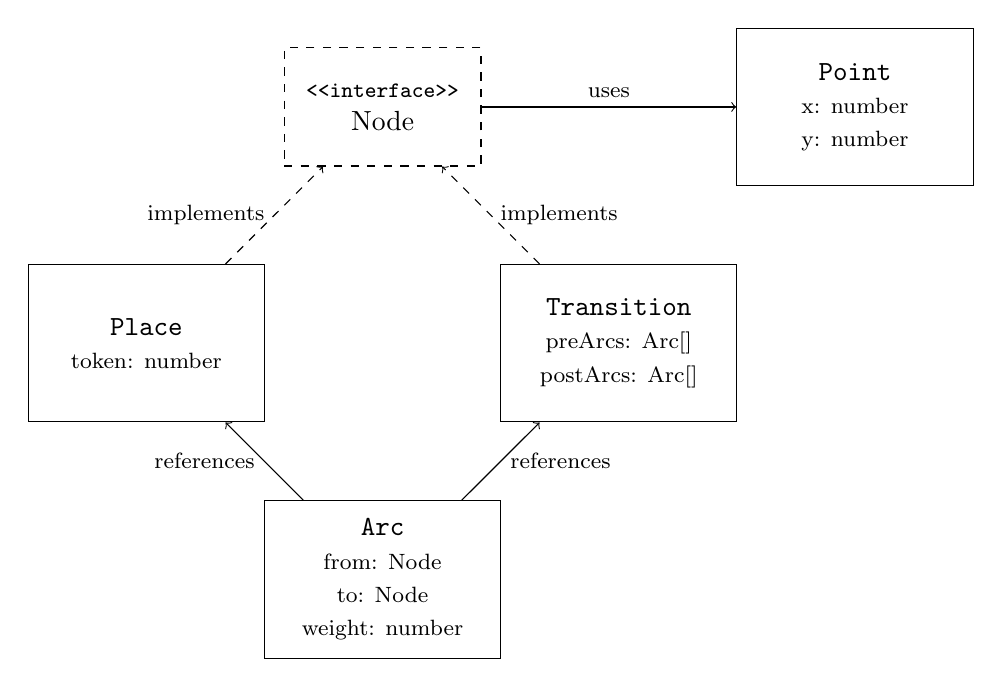
\begin{tikzpicture}[
        class/.style={rectangle, draw, minimum width=3cm, minimum height=2cm, align=center},
        interface/.style={rectangle, draw, dashed, minimum width=2.5cm, minimum height=1.5cm, align=center},
    ]
        % Classes
        \node[interface] (node) at (0, 3) {\footnotesize \texttt{<<interface>>}\\Node};
        \node[class] (place) at (-3, 0) {\texttt{Place}\\{\footnotesize token: number}};
        \node[class] (transition) at (3, 0) {\texttt{Transition}\\{\footnotesize preArcs: Arc[]}\\{\footnotesize postArcs: Arc[]}};
        \node[class] (arc) at (0, -3) {\texttt{Arc}\\{\footnotesize from: Node}\\{\footnotesize to: Node}\\{\footnotesize weight: number}};
        \node[class] (point) at (6, 3) {\texttt{Point}\\{\footnotesize x: number}\\{\footnotesize y: number}};
        
        % Relationships
        \draw[->, dashed] (place) -- (node) node[midway, left] {\footnotesize implements};
        \draw[->, dashed] (transition) -- (node) node[midway, right] {\footnotesize implements};
        \draw[->] (arc) -- (place) node[midway, left] {\footnotesize references};
        \draw[->] (arc) -- (transition) node[midway, right] {\footnotesize references};
        \draw[->] (node) -- (point) node[midway, above] {\footnotesize uses};
    \end{tikzpicture}
    \caption{Petri net element class relationships}
    \label{fig:elements-class-diagram}
\end{figure}

\section{Summary}
\label{sec:elements-summary}

The \textbf{Petri Net Elements} are the fundamental data objects that define any Petri net:

\begin{itemize}
    \item \textbf{Place}: Holds tokens, represents states/conditions
    \item \textbf{Transition}: Represents actions, fires when enabled
    \item \textbf{Arc}: Connects places and transitions, defines token flow
    \item \textbf{Point}: Stores canvas coordinates for positioning
    \item \textbf{Node interface}: Common contract for places and transitions
\end{itemize}

These objects are the ``things'' you manipulate when designing a Petri net. But how does the application manage a \textit{collection} of these elements? How does it track all places, transitions, and arcs in your entire net? That's the role of the \textbf{Data Service}, which we explore in the next chapter.
